%================ch3======================================
\chapter{Tools for Genomic Data Analysis}\label{ch:ch4}

\section{Basic Local Alignment Search Tool(BLAST)}  
\text{BLAST} finds regions of similarity between biological sequences. The program compares nucleotide or protein sequences to sequence databases and calculates the statistical significance.(\url{https://blast.ncbi.nlm.nih.gov/Blast.cgi}) 
To overcome the limitations of the classic alignment algorithms, which are usually used for rather short sequences, new methods and heuristics were developed. By heuristic algorithm we imply a non-exact solution, which works faster than exact algorithms (sometimes much faster) and provides biologically meaningful results \cite{seq2018}.
 

\section{FastQC} 
FastQC aims to provide a simple way to do some quality control checks on raw sequence data coming from high throughput sequencing pipelines. It provides a modular set of analyses which you can use to give a quick impression of whether your data has any problems of which you should be aware before doing any further analysis (Figure~\ref{fig:fastqc}).  (\url{https://www.bioinformatics.babraham.ac.uk/projects/fastqc/}) 

The main functions of FastQC are: 
\begin{enumerate}
	\item Import of data from BAM, SAM or FastQ files (any variant) 
	\item Providing a quick overview to tell you in which areas there may be problems
	\item Summary graphs and tables to quickly assess your data
	\item Export of results to an HTML based permanent report
	\item Offline operation to allow automated generation of reports without running the interactive application
	
\end{enumerate}

\begin{figure}
	\centering
	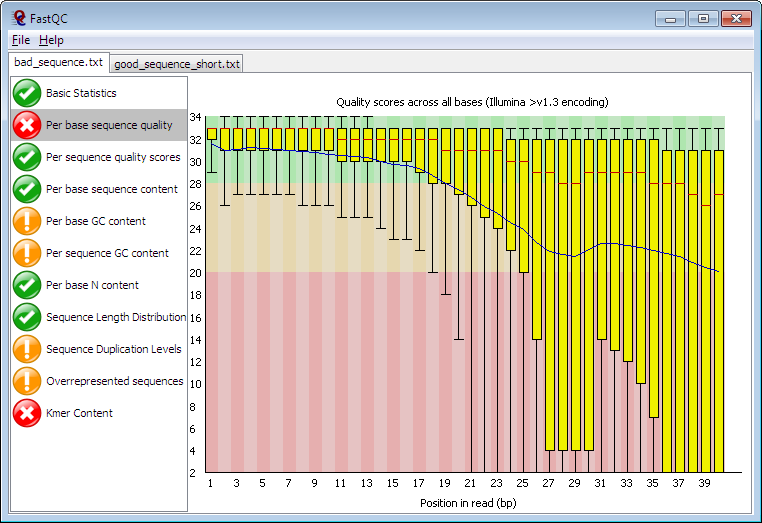
\includegraphics[width=0.7\linewidth]{fastqc}
	\caption{Example of FastQC Result}
	\label{fig:fastqc}
\end{figure} 

\section{MultiQC} 
MultiQC is a reporting tool that parses summary statistics from results and log files generated by other bioinformatics tools. MultiQC doesn't run other tools for you - it's designed to be placed at the end of analysis pipelines or to be run manually when you've finished running your tools. (Figure~\ref{fig:fastqc})

When you launch MultiQC, it recursively searches through any provided file paths and finds files that it recognises. It parses relevant information from these and generates a single stand-alone HTML report file. It also saves a directory of data files with all parsed data for further downstream use. (Figure~\ref{fig:multiqc}) (\url{https://multiqc.info/}) 

\begin{figure}
	\centering
	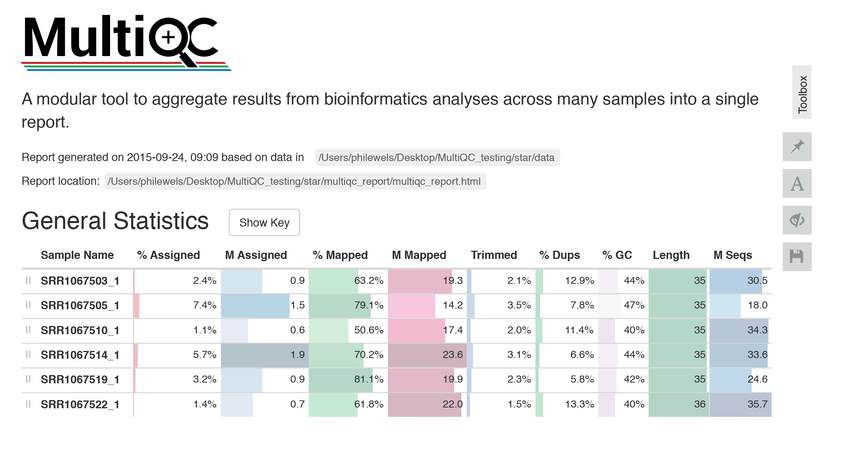
\includegraphics[width=0.7\linewidth]{multiqc}
	\caption{Example of MultiQC Report}
	\label{fig:multiqc}
\end{figure} 


\section{R Programming}
The aim of computational genomics is to provide biological interpretation and insights from high dimensional genomics data. Generally speaking, it is similar to any other kind of data analysis endeavor but often times doing computational genomics will require domain specific knowledge and tools.

As new high-throughput experimental techniques are on the rise, data analysis capabilities are sought-after features for researchers. The aim of this chapter is to first familiarize the readers with data analysis steps and then provide basics of R programming within the context of genomic data analysis. R is a free statistical programming language that is popular among researchers and data miners to build software and analyze data. Although basic R programming tutorials are easily accessible, we are aiming to introduce the subject with the genomic context in the background. The examples and narrative will always be from real-life situations when you try to analyze genomic data with R. We believe tailoring material to the context of genomics makes a difference when learning this programming language for sake of analyzing genomic data. (\url{https://www.r-project.org/about.html})


\section{Python}
Python is a general-purpose programming language conceived in 1989 by Dutch programmer Guido van Rossum.Python is free and open source, with development coordinated through the Python Software Foundation.

Python has experienced rapid adoption in the last decade and is now one of the most commonly used programming languages. Python is also used widely in the field of bioinformatics, computational genomics, genomics and computational drug development. \url{https://www.python.org/} 


\section{Biopython} 
Biopython is a set of freely available tools for biological computation written in Python by an international team of developers. (\url{https://biopython.org/}) 

\section{Sciki-bio} 
scikit-bio™ is an open-source, BSD-licensed, python package providing data structures, algorithms, and educational resources for bioinformatics. (\url{http://scikit-bio.org/}) 

\section{Bioconductor}
Bioconductor provides tools for the analysis and comprehension of high-throughput genomic data. Bioconductor uses the R statistical programming language, and is open source and open development. It has two releases each year, and an active user community. (\url{https://www.bioconductor.org/}) 

